%author:        Troels
%1st review:    Sass
\section{Radio Frequency Module} \label{rfmodule}
To achieve wireless communication between the devices an \gls{rf} module is used.
The module used in this project communicates at 433 MHz; its datasheet \cite{RFRX, RFTX} specifies the range is 20 to 200 meters, depending on the input voltage, which ranges from 3.5 to 12 volts. 
The Arduino provides 3.3 volts and 5 volts output, and the 5 volts output will be used.
The largest bandwidth is 4 kilobytes/second. 
The signal is sent using \gls{ask} which will be further explained in \myref[name]{subsub:ask}.
These values will be tested in \myref[name]{sec:hardware_tests} to ensure the reliability of the information. 

\bigskip \noindent
The \gls{rf} system consists of a \gls{tx} and a \gls{rx}, see \myref{fig:arduino_rf}.
The \gls{tx} module has three connector pins.
The pins are VCC, power supply pin, GND, ground pin, and DATA.
The DATA pin is turned on by having the same difference in voltage between GND and DATA as VCC and GND. 
The \gls{rx} module has the same pins as the transmitting module, but the DATA pins are being read from instead of transmitted to.

\begin{figure}[h] 
\vspace{-5pt} 
\centering
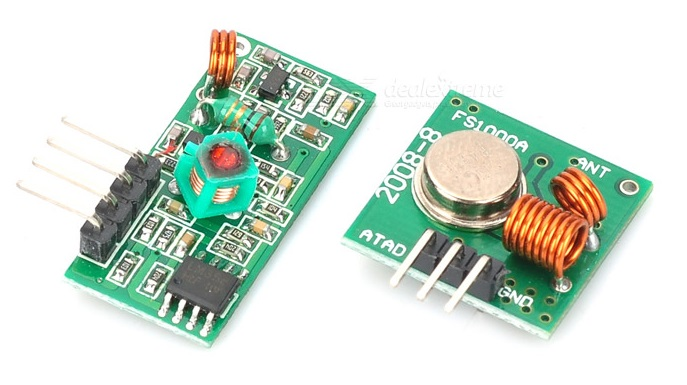
\includegraphics[width=0.4\textwidth]{Figures/arduino_rf.jpg}
\vspace{-5pt} 
\caption{The 433MHz \gls{rf} receiver (left) and transmitter (right)}
\label{fig:arduino_rf}
\vspace{-5pt}    
\end{figure}

\subsection{Antenna}
It is possible to attach an antenna to both \gls{rf}-modules. 
The benefit of using an antenna is an improvement in both greatest distance and reliability of transmissions.
Attaching an antenna is done by soldering the antenna to the ANT port on both the receiver and the transmitter. 
In \myref{fig:arduino_rf} these are visible; one in the upper left corner on the receiver and one in the upper right corner on the transmitter. 

A wire acts like a monopole antenna which works by acting like an open resonator for the signal, its length can affect its effect. 
Candidates for the length of this can be calculated based on the frequency of the signal.
For the \gls{rf}-modules, this is 433 MHz.
The formula for a quarter-monopole antenna is: 
\begin{equation} \label{QMA}
l = \frac{c}{f \times 4}
\end{equation}
where c is the speed of light, and f is the frequency of the wave.
The formula for a half-monopole antenna is: 

\begin{equation}
l = \frac{c}{f \times 2}
\end{equation}

\noindent
Using the frequency, 433 MHz, the quarter- and half-monopole antenna lengths are 17.3 cm and 34.6 cm, see \cite{AntennaLength} for more information.
The efficiency of using 17.3 cm antennas will be tested in \myref[name]{cha:radio_frequency_module_reception_test}.

\subsection{Amplitude Shift Keying}\label{subsub:ask}
As mentioned the \gls{rf} module sends its signal using \gls{ask}.
\gls{ask} is a form of modulation where the digital input is a radio wave where the digital high (also known as \enquote*{1}) is a greater amplitude than the digital low (also known as \enquote*{0}).
To use \gls{ask} the devices must be synchronised meaning that the time period of a single bit must be known by the receiver, in order for it to demodulate it. 
In \myref{fig:ask} is an example of how a radio wave would look like while using \gls{ask}, here the period for each signal is twice the period of the wave. See \cite{ASKnFSK} for more information.  

\tikzfigure{ASK.tex}{\gls{ask}: Digital values are signaled by the amplitude of the radio wave.}{ask}
